\documentclass[10.5pt,a4paper]{article}

\usepackage[T1]{fontenc}
\usepackage[utf8]{inputenc}
\usepackage{libertinus}
\usepackage{libertinust1math}
\usepackage[scaled=0.83]{beramono}
\usepackage[margin=2.3cm,top=2.2cm,bottom=2.4cm]{geometry}
\usepackage{microtype}
\usepackage{amsmath,amsthm,mathtools}
\usepackage{booktabs,tabularx,array}
\usepackage{graphicx}
\usepackage{xcolor}
\usepackage{tikz}
\usetikzlibrary{arrows.meta,positioning,fit,calc}
\usepackage[ruled,vlined,linesnumbered]{algorithm2e}
\usepackage{enumitem}
\usepackage[hidelinks]{hyperref}
\usepackage[capitalise,nameinlink]{cleveref}
\usepackage{caption}
\captionsetup{font=small,labelfont=bf}

\definecolor{cairn}{HTML}{2a78d6}
\definecolor{naive}{HTML}{eb6834}
\definecolor{ink2}{HTML}{52514e}
\hypersetup{colorlinks,linkcolor=cairn!80!black,citecolor=cairn!80!black,urlcolor=cairn!80!black}

\theoremstyle{plain}
\newtheorem{theorem}{Theorem}
\newtheorem{lemma}[theorem]{Lemma}
\newtheorem{proposition}[theorem]{Proposition}
\newtheorem{corollary}[theorem]{Corollary}
\theoremstyle{definition}
\newtheorem{definition}[theorem]{Definition}
\newtheorem{remark}[theorem]{Remark}
\crefname{theorem}{Theorem}{Theorems}
\crefname{lemma}{Lemma}{Lemmas}
\crefname{proposition}{Proposition}{Propositions}

\newcommand{\F}{\mathbb{F}}
\newcommand{\Fp}{\mathbb{F}_p}
\newcommand{\ip}[2]{\langle #1,#2\rangle}
\newcommand{\TV}{\mathrm{TV}}
\newcommand{\Hinf}{\mathrm{H}_\infty}
\newcommand{\Skew}{\mathrm{Skew}_\ell(\Fp)}
\newcommand{\Enc}{\mathsf{IPEnc}}
\newcommand{\getsr}{\xleftarrow{\$}}
\newcommand{\cairn}{\textsc{Cairn}}
\newcommand{\code}[1]{\texttt{#1}}
\SetKwInput{KwIn}{Input}
\SetKwInput{KwOut}{Output}
\SetKwComment{Comment}{\color{ink2}$\triangleright$\ }{}

% generated by paper/figures.py from results/*.json; do not edit
\newcommand{\DudectMulCairn}{1.6}
\newcommand{\SamplesMulCairn}{2{,}000{,}000}
\newcommand{\DudectMulNaive}{11{,}848.1}
\newcommand{\SamplesMulNaive}{2{,}000{,}000}
\newcommand{\DudectInvCairn}{1.5}
\newcommand{\SamplesInvCairn}{200{,}000}
\newcommand{\DudectInvNaive}{2{,}964.1}
\newcommand{\SamplesInvNaive}{200{,}000}
\newcommand{\DudectRecCairn}{1.4}
\newcommand{\SamplesRecCairn}{200{,}000}
\newcommand{\DudectRecNaive}{1{,}107.6}
\newcommand{\SamplesRecNaive}{200{,}000}
\newcommand{\BenchMul}{25\,ns}
\newcommand{\BenchInv}{2.2\,\textmu s}
\newcommand{\BenchSplit}{63.6\,\textmu s}
\newcommand{\BenchCombine}{9.3\,\textmu s}
\newcommand{\BenchCheat}{45.9\,\textmu s}
\newcommand{\BenchRefresh}{133.3\,\textmu s}
\newcommand{\BenchLocal}{15.9\,\textmu s}
\newcommand{\BenchDelta}{28.2\,\textmu s}
\newcommand{\SecrecyDealings}{77{,}525}
\newcommand{\AmdPairs}{13{,}432{,}176}

\makeatletter
\newcommand{\rows}[1]{\@@input generated/#1.tex }
\makeatother

\title{\textbf{\cairn{}}: Information-Theoretic, Leakage-Resilient\\Threshold Custody of Master Keys from Linear Algebra over $\F_{2^{127}-1}$}
\author{Ahmedouyahya\\[2pt]\small Mathematics for Systems Security, Cryptographer track}
\date{November 2026}

\begin{document}
\maketitle

\begin{abstract}
\noindent
A master key is exposed through five different windows: \emph{at rest} (a stolen backup), \emph{over time} (an attacker who collects pieces patiently), \emph{in memory} (cold boot, swap, partial memory disclosure), \emph{during reconstruction} (timing and cache side channels) and \emph{under manipulation} (a custodian who lies). We present \cairn{}, a $t$-of-$n$ custody scheme that closes all five with one algebraic toolbox and \emph{no computational assumption at all}: no block cipher, no hash function, no discrete logarithm. The key is encoded into the Mersenne field $\Fp$, $p=2^{127}-1$, armored with an algebraic manipulation detection tag, shared with a Vandermonde system, and every share coordinate is stored as an inner product $\ip{L}{R}$ of two vectors kept in separate memory regions. Shares are re-randomized by Gibbs steps built from random skew-symmetric matrices, and moved to fresh sharings by zero-polynomial refreshes. We prove perfect secrecy against $t-1$ custodians, tamper detection with error at most $(k+1)/p\approx 2^{-125}$, resilience to $379$ bits of arbitrary split-state leakage per share coordinate at advantage $2^{-128}$, and security against mobile adversaries. We report our own cryptanalysis, including a cross-epoch attack on the natural two-step refresh that we found and fixed. Every claim is backed by an exact or statistical experiment that \code{make verify} reproduces: exhaustive enumeration in small fields (\SecrecyDealings{} dealings, \AmdPairs{} secret/error pairs), byte-identical agreement with an independent reference implementation, a fixed-versus-random timing test (CAIRN $|t|\le\DudectMulCairn$, textbook baseline $|t|$ up to \DudectMulNaive{}), an assembly audit and memory-safety checks. The implementation is a \code{no\_std}, \code{unsafe}-free Rust core with a hardened command line tool.
\end{abstract}

\section{Introduction}\label{sec:intro}

Whoever holds a master key holds everything it protects: a signing key for software releases, the root of a password manager, the key-encryption key of a database. The classical answer to ``who should hold it'' is Shamir secret sharing~\cite{shamir79}: split the key into $n$ shares so that any $t$ recover it and any $t-1$ reveal nothing. Shamir's scheme is perfect, but only \emph{as mathematics}. Deployed, it leaves five windows open, and each has been exploited in practice or in the literature.

\begin{enumerate}[leftmargin=*,label=\textbf{W\arabic*.},itemsep=1pt]
\item \textbf{At rest.} Shares are files; files get copied.
\item \textbf{Over time.} A \emph{mobile} adversary~\cite{ostrovsky91} who steals one share a month eventually holds $t$ shares of the same polynomial.
\item \textbf{In memory.} Shares and the key sit in RAM, swap and core dumps, readable by cold-boot attacks~\cite{halderman08} or partial memory disclosure.
\item \textbf{During reconstruction.} Variable-time arithmetic leaks through timing and cache channels~\cite{kocher96}.
\item \textbf{Under manipulation.} A single cheating custodian who submits a modified share makes everyone else recover a wrong key while she computes the right one (Tompa and Woll~\cite{tompa88}).
\end{enumerate}

\paragraph{Contributions.} \cairn{} is a complete custody scheme in which each window is closed by a layer with a proof and a measurement (\cref{tab:windows}).
\begin{itemize}[leftmargin=*,itemsep=1pt]
\item A construction that uses only linear algebra and polynomial arithmetic over $\Fp$, $p=2^{127}-1$: algebraic manipulation detection (AMD)~\cite{cramer08}, Vandermonde sharing, inner-product split-state storage~\cite{davi10,dziembowski11}, and a new inversion-free refresh by random skew-symmetric matrices (\cref{sec:construction}).
\item Unconditional security theorems with explicit bounds, proved in full (\cref{sec:security}), including a self-contained proof of the split-state leakage bound (\cref{thm:leakage}) and an exact analysis of cross-epoch leakage of the refresh (\cref{lem:refresh}).
\item Cryptanalysis of our own design (\cref{sec:cryptanalysis}): a complete break of the obvious two-step refresh, the limits of any keyless robust scheme, and attacks on parsing, timing and process memory.
\item Evidence for every claim (\cref{sec:evaluation}): exhaustive verification at small parameters through the production code path, cross-implementation known-answer tests, dudect-style timing tests, ctgrind, an assembly audit and Miri.
\end{itemize}

\begin{table}[t]
\centering\small
\begin{tabularx}{\textwidth}{@{}l l X l@{}}
\toprule
Window & Layer & Guarantee & Evidence\\
\midrule
W1 at rest & L3 Vandermonde sharing & $t-1$ shares independent of the key (\cref{thm:secrecy}) & exhaustive, \cref{tab:secrecy}\\
W2 over time & L5 zero-sharing refresh & mobile adversary learns nothing (\cref{thm:mobile}) & demo, \cref{sec:attack-mobile}\\
W3 in memory & L4 split-state storage & $2^{-128}$ advantage under 379 bits of leakage (\cref{thm:leakage}) & exact, \cref{fig:leakage}\\
W3 over refreshes & L4 skew-symmetric refresh & cross-epoch advantage $p^{-(\ell-1)}$ (\cref{lem:refresh}) & exact, \cref{tab:refresh}\\
W4 reconstruction & L6 constant-time combine & no secret-dependent branch, address or latency & dudect, ctgrind, asm\\
W5 manipulation & L2 AMD armor & wrong key accepted w.p.\ $\le (k+1)/p$ (\cref{thm:robust}) & exhaustive, \cref{tab:amd}\\
\bottomrule
\end{tabularx}
\caption{Vulnerability windows of a master key and how \cairn{} closes them.}\label{tab:windows}
\end{table}

\section{Preliminaries}\label{sec:prelim}

\paragraph{Field.} Let $p=2^{127}-1$, a Mersenne prime, and $\F=\Fp$. Since $2^{127}\equiv 1 \pmod p$, a 254-bit product $h\cdot 2^{128}+l$ reduces as $l\bmod 2^{127} + \lfloor l/2^{127}\rfloor + 2h$ followed by one conditional subtraction, which we implement with a mask. Inversion is $x^{-1}=x^{p-2}$ (Fermat) with the \emph{public} exponent $p-2$, so its operation sequence does not depend on $x$; we set $0^{-1}=0$. All elements are kept in canonical form $[0,p)$, and encodings that are not canonical are rejected, so every element has exactly one byte representation.

\paragraph{Notation.} $[n]=\{1,\dots,n\}$. For $u,v\in\F^\ell$, $\ip{u}{v}=\sum_i u_iv_i$ and $u^\perp=\{v:\ip{u}{v}=0\}$. $\Skew$ is the set of $\ell\times\ell$ matrices with $A^\top=-A$. For distributions $P,Q$ on a finite set, $\TV(P,Q)=\frac12\sum_z|P(z)-Q(z)|$; the advantage of any distinguisher between $P$ and $Q$ is at most $\TV(P,Q)$. $X\getsr S$ denotes uniform sampling. Characters of $(\F,+)$ are $\psi_a(z)=\omega^{az}$ with $\omega=e^{2\pi i/p}$.

\paragraph{Threat model.} The adversary may (A1) steal up to $t-1$ share files; (A2) be \emph{mobile}, stealing up to $t-1$ shares in each refresh epoch, where a custodian corrupted during a refresh counts for both epochs; (A3) control up to $t-1$ custodians and submit arbitrary share files for them at combination time; (A4) obtain adaptive leakage of at most $\lambda_L$ bits from the $L$ memory region and $\lambda_R$ bits from the $R$ region of any share (\emph{split-state} model); (A5) obtain one storage half before a refresh and the other half after it; (A6) measure the timing and cache behaviour of the combiner; (A7) feed malformed files. We trust: (T1) the dealer during dealing, (T2) the combiner during combination (it outputs the key by definition), (T3) the operating system's random number generator, (T4) confidentiality of refresh deltas in transit, and (T5) the binding between a custodian and her share index at combination time (the roster; \cref{prop:keyless} shows that no keyless scheme can avoid an assumption of this kind).

\section{The \cairn{} construction}\label{sec:construction}

\begin{figure}[t]
\centering
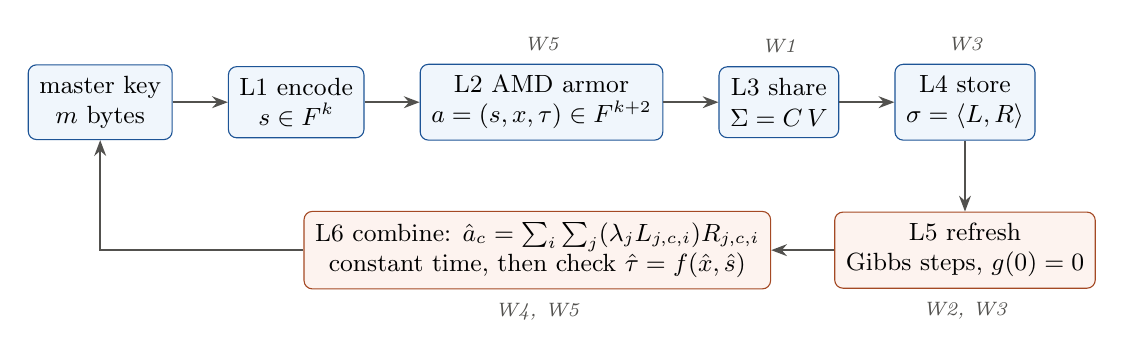
\begin{tikzpicture}[
  font=\small,
  box/.style={draw=cairn!70!black, fill=cairn!7, rounded corners=3pt, minimum height=9mm, align=center, inner sep=4pt},
  lab/.style={font=\scriptsize\itshape, text=ink2, align=center},
  ar/.style={-{Stealth[length=2mm]}, draw=ink2, thick}]
\node[box] (key) {master key\\$m$ bytes};
\node[box, right=7mm of key] (enc) {L1 encode\\$s\in\F^k$};
\node[box, right=7mm of enc] (amd) {L2 AMD armor\\$a=(s,x,\tau)\in\F^{k+2}$};
\node[box, right=7mm of amd] (sh) {L3 share\\$\Sigma = C\,V$};
\node[box, right=7mm of sh] (ip) {L4 store\\$\sigma=\ip{L}{R}$};
\draw[ar] (key) -- (enc); \draw[ar] (enc) -- (amd); \draw[ar] (amd) -- (sh); \draw[ar] (sh) -- (ip);
\node[box, below=9mm of ip, fill=naive!8, draw=naive!70!black] (ref) {L5 refresh\\Gibbs steps, $g(0)=0$};
\node[box, left=8mm of ref, fill=naive!8, draw=naive!70!black] (comb) {L6 combine: $\hat a_c=\sum_{i}\sum_{j}(\lambda_jL_{j,c,i})R_{j,c,i}$\\constant time, then check $\hat\tau=f(\hat x,\hat s)$};
\draw[ar] (ip) -- (ref); \draw[ar] (ref) -- (comb);
\draw[ar] (comb.west) -| (key.south);
\node[lab, above=0.5mm of amd] {W5};
\node[lab, above=0.5mm of sh] {W1};
\node[lab, above=0.5mm of ip] {W3};
\node[lab, below=0.5mm of ref] {W2, W3};
\node[lab, below=0.5mm of comb] {W4, W5};
\end{tikzpicture}
\caption{The six layers of \cairn{} and the windows (W1 to W5) they close.}\label{fig:pipeline}
\end{figure}

\paragraph{L1, encoding.} A secret of $m\le 65535$ bytes is prefixed with its 16-bit length, padded with zeros to a multiple of 15 bytes and cut into $k$ big-endian 120-bit limbs $s_1,\dots,s_k<2^{120}<p$. The map is injective, and decoding rejects any vector that is not exactly an encoding. A parameter $k_{\min}$ pads short secrets to a fixed number of limbs so that $k$, which is public, does not reveal the length. A 32-byte key gives $k=3$.

\paragraph{L2, AMD armor~\cite{cramer08}.} Draw $x\getsr\F$ and set
\[
\tau = f(x,s) = x^{k+2}+\sum_{i=1}^k s_i x^i, \qquad a = (s_1,\dots,s_k,x,\tau)\in\F^{D},\quad D=k+2.
\]
The tag is evaluated by Horner's rule as $x\cdot(s_1+x(s_2+\dots+x(s_k+x\cdot x)))$: exactly $k+1$ multiplications whatever the values.

\paragraph{L3, sharing.} For each component $c\in[D]$ draw $f_c(X)=a_c+\sum_{m=1}^{t-1} r_{c,m}X^m$ with $r_{c,m}\getsr\F$. In matrix form, with $C\in\F^{D\times t}$ the coefficient matrix and $V=[\,j^m\,]_{0\le m<t,\ j\in[n]}$ a Vandermonde matrix, the share matrix is $\Sigma = CV$; share $j$ is the column $\sigma_j=(f_c(j))_c$.

\paragraph{L4, split-state storage.} Each coordinate $\sigma_{j,c}$ is stored as a pair $(L,R)\in\F^\ell\times\F^\ell$ with $\ip{L}{R}=\sigma_{j,c}$, produced by \cref{alg:ipenc}. All $L$ vectors of a share live in one memory region and file section, all $R$ vectors in another.

\paragraph{L5, refresh.} \Cref{alg:refresh} re-randomizes a pair without computing its value; \cref{alg:proactive} moves all custodians to a fresh sharing of the same key.

\paragraph{L6, combination.} \Cref{alg:combine} interpolates at zero in constant time and checks the AMD tag. Lagrange coefficients depend only on the public indices.

\begin{algorithm}[t]
\caption{$\Enc(\sigma)$: inner-product encoding}\label{alg:ipenc}
\KwIn{$\sigma\in\F$, dimension $\ell\ge 2$}
$L_1\getsr\F\setminus\{0\}$;\quad $L_2,\dots,L_\ell\getsr\F$;\quad $R_2,\dots,R_\ell\getsr\F$\;
$R_1\gets(\sigma-\sum_{i\ge2}L_iR_i)\cdot L_1^{\,p-2}$\Comment*[r]{inverts a random value, constant time}
\Return{$(L,R)$}\Comment*[r]{uniform on $S_\sigma=\{(L,R):\ip{L}{R}=\sigma,\ L_1\neq0\}$}
\end{algorithm}

\begin{algorithm}[t]
\caption{$\mathsf{Refresh}(L,R)$: three Gibbs half-steps}\label{alg:refresh}
$A,B,C\getsr\Skew$\Comment*[r]{$\ell(\ell-1)/2$ field elements each}
$L\gets L+AR$\Comment*[r]{$\ip{AR}{R}=0$, so $\ip{L}{R}$ is unchanged}
$R\gets R+BL$\;
$L\gets L+CR$\;
\Return{$(L,R)$}
\end{algorithm}

\begin{algorithm}[t]
\caption{$\mathsf{ProactiveRefresh}$ for a dealing with parameters $(t,n,D)$}\label{alg:proactive}
\textbf{Coordinator:} for $c\in[D]$ draw $g_c(X)=\sum_{m=1}^{t-1}u_{c,m}X^m$, $u_{c,m}\getsr\F$; send $\delta_j=(g_c(j))_c$ to custodian $j$ confidentially\;
\textbf{Custodian $j$:} for $c\in[D]$: $R_{j,c,1}\gets R_{j,c,1}+\delta_{j,c}\cdot L_{j,c,1}^{-1}$;\ $(L_{j,c},R_{j,c})\gets\mathsf{Refresh}(L_{j,c},R_{j,c})$\;
increment the epoch; erase $\delta_j$\;
\end{algorithm}

\begin{algorithm}[t]
\caption{$\mathsf{Combine}(\text{shares } \mathcal{S})$}\label{alg:combine}
check that all shares have the same dealing identifier, parameters and epoch, distinct indices in $[n]$, and $|\mathcal S|\ge t$\;
\ForEach{$t$-subset $T\subseteq\mathcal S$ in lexicographic order (at most $2^{16}$)}{
  $\lambda_j\gets\prod_{m\in T\setminus\{j\}} m\,(m-j)^{-1}$ for $j\in T$\Comment*[r]{public}
  \For{$c\in[D]$}{$\hat a_c\gets\sum_{i=1}^{\ell}\sum_{j\in T}(\lambda_j L_{j,c,i})\,R_{j,c,i}$\Comment*[r]{no single share is ever formed}}
  \If{$\mathsf{ct\_eq}(\hat\tau, f(\hat x,\hat s))$ \textnormal{(declassified verdict)}}{
     report as inconsistent every $u\notin T$ for which $(T\setminus\{\min T\})\cup\{u\}$ fails the check\;
     \Return{$\mathsf{Decode}(\hat s)$}}
}
\Return{$\bot$}
\end{algorithm}

\section{Security analysis}\label{sec:security}

\begin{theorem}[Correctness]\label{thm:correct}
For every secret and every $t$-subset $T$ of honest shares of the same epoch, \cref{alg:combine} returns the secret.
\end{theorem}
\begin{proof}
Every operation of \cref{alg:ipenc,alg:refresh} preserves $\ip{L}{R}$: \cref{alg:ipenc} by construction, and each line of \cref{alg:refresh} adds a vector orthogonal to the other half because $\ip{Mw}{w}=w^\top M^\top w=-w^\top Mw$ forces $\ip{Mw}{w}=0$ for skew-symmetric $M$ when $p$ is odd. In \cref{alg:proactive}, $\ip{L}{R+(\delta/L_1)e_1}=\ip{L}{R}+\delta$, and $\sum_{j\in T}\lambda_j g_c(j)=g_c(0)=0$, so refreshes do not change the interpolated value. Hence $\hat a_c=\sum_{j\in T}\lambda_jf_c(j)=f_c(0)=a_c$ by Lagrange interpolation, the tag verifies, and $\mathsf{Decode}$ inverts L1.
\end{proof}

\subsection{Secrecy at rest and over time}

\begin{theorem}[Perfect secrecy]\label{thm:secrecy}
For every set $B\subseteq[n]$ with $|B|\le t-1$, the joint distribution of the share files $(\text{share}_j)_{j\in B}$ is the same for every secret.
\end{theorem}
\begin{proof}
Fix a component $c$. The values on $B$ are $f_c(j)=a_c+\sum_{m=1}^{t-1}r_{c,m}j^m$, that is $a_c\mathbf 1+V_B r_c$ with $V_B=[j^m]_{j\in B,\,1\le m<t}$. Now $V_B=\mathrm{diag}(j)_{j\in B}\,W$, where $W=[j^{m-1}]$ is a $|B|\times(t-1)$ Vandermonde matrix on distinct points, hence of full row rank, and $\mathrm{diag}(j)$ is invertible because $0\notin B$. So $r_c\mapsto V_Br_c$ is onto $\F^{|B|}$ and maps the uniform distribution to the uniform distribution; the values are uniform whatever $a_c$. Components use independent coefficients, and the files are randomized functions of the values, the public parameters and the random identifier.
\end{proof}

\begin{theorem}[Mobile adversary]\label{thm:mobile}
Let $B_e$ be the custodians corrupted in epoch $e$, with $|B_e|\le t-1$, where a custodian corrupted during the refresh from $e-1$ to $e$ belongs to both $B_{e-1}$ and $B_e$ and also sees her delta. Assume deltas are confidential and erased. Then the adversary's view over any number of epochs is independent of the secret.
\end{theorem}
\begin{proof}
Write $f^{(e)}_c$ for the epoch-$e$ polynomial, so $f^{(e)}_c=f^{(e-1)}_c+g^{(e-1)}_c$ with $g^{(e-1)}_c(0)=0$ fresh. We show by induction that the epoch-$e$ part of the view is independent of the secret given the earlier view. Epoch 0 is \cref{thm:secrecy}. For $e\ge1$, the vector $(g^{(e-1)}_c(j))_{j\in B_e}$ is uniform on $\F^{|B_e|}$ (same Vandermonde argument, as $|B_e|\le t-1$) and independent of everything before. The new values are: for $j\in B_e\cap B_{e-1}$, old value plus seen delta, a function of the earlier view and of uniform fresh values; for $j\in B_e\setminus B_{e-1}$, $f^{(e-1)}_c(j)+g^{(e-1)}_c(j)$, which is uniform and independent of the earlier view because the second term is a fresh uniform coordinate that appears nowhere else in the view. Storage encodings are fresh randomized functions of these values.
\end{proof}

\subsection{Tamper detection}

\begin{lemma}[AMD bound~\cite{cramer08}]\label{lem:amd}
Let $k+2\not\equiv0\pmod p$. For every $s\in\F^k$ and every non-zero $\Delta=(d,e,g)\in\F^k\times\F\times\F$,
$\Pr_{x\getsr\F}\big[\,\tau+g=f(x+e,s+d)\,\big]\le\frac{k+1}{p}$, where $\tau=f(x,s)$.
\end{lemma}
\begin{proof}
The event is $P(x)=0$ for $P(x)=f(x+e,s+d)-f(x,s)-g$. If $e\neq0$, the coefficient of $x^{k+1}$ in $(x+e)^{k+2}-x^{k+2}$ is $(k+2)e\neq0$ and the other terms have degree at most $k$, so $P$ has degree exactly $k+1$ and at most $k+1$ roots. If $e=0$, $P(x)=\sum_i d_ix^i-g$ has degree at most $k$ and is the zero polynomial only if $d=0$ and $g=0$, i.e.\ $\Delta=0$.
\end{proof}

\begin{theorem}[Robustness]\label{thm:robust}
Let at most $t-1$ custodians be corrupted (A3), each submitting an arbitrary file under her own index (T5). Then \cref{alg:combine} returns either the correct secret or $\bot$, except with probability at most $N\,(k+1)/p$, where $N\le 2^{16}+n$ is the number of subsets it evaluates.
\end{theorem}
\begin{proof}
For one subset $T$ the reconstruction is linear: $\hat a=a+\sum_{j\in T\cap B}\lambda_j(\sigma'_j-\sigma_j)=a+\Delta_T$. The corrupted parties choose $\sigma'_j$ from their view, which by \cref{thm:secrecy} is independent of $a$; in particular, for any fixed $s$, $\Delta_T$ is independent of $x$. If $\Delta_T=0$ the output is correct. Otherwise, by \cref{lem:amd}, the tag verifies with probability at most $(k+1)/p$. A union bound over the evaluated subsets concludes. Since every $t$-subset contains an honest share when $|B|\le t-1$, the adversary cannot replace the reconstruction by a value of her choice.
\end{proof}

With $k=3$ the bound is $2^{-125}$ per subset and below $2^{-108}$ for the whole search. The same argument shows that shares from different epochs combine to the correct secret or to $\bot$ except with probability $(k+1)/p$: the mixture adds $\sum_j\lambda_j(g(j)-g'(j))$, a function of refresh randomness only.

\subsection{Leakage from storage}

\begin{lemma}[Inner-product extractor]\label{lem:lindsey}
Let $\mathcal A,\mathcal B\subseteq\F^\ell$ be non-empty and $X\getsr\mathcal A$, $Y\getsr\mathcal B$ independent. Then
$\TV\big(\ip XY,\,U_\F\big)\le\frac12\sqrt{p^{\ell+1}/(|\mathcal A||\mathcal B|)}$.
\end{lemma}
\begin{proof}
For $a\neq0$, by Cauchy-Schwarz and then extending the sum to all of $\F^\ell$,
\[
\Big|\sum_{x\in\mathcal A}\sum_{y\in\mathcal B}\psi_a(\ip xy)\Big|^2\le|\mathcal A|\sum_{x\in\F^\ell}\Big|\sum_{y\in\mathcal B}\psi_a(\ip xy)\Big|^2=|\mathcal A|\sum_{y,y'\in\mathcal B}\sum_{x\in\F^\ell}\psi_a(\ip x{y-y'})=|\mathcal A||\mathcal B|p^\ell,
\]
so $|\mathbb E\,\psi_a(\ip XY)|\le\sqrt{p^\ell/(|\mathcal A||\mathcal B|)}$ (Lindsey's lemma~\cite{chor88}). Writing $D=P_{\ip XY}-U_\F$, Parseval gives $\sum_z D(z)^2=\frac1p\sum_{a\neq0}|\mathbb E\,\psi_a(\ip XY)|^2$, and Cauchy-Schwarz gives $\TV=\frac12\sum_z|D(z)|\le\frac12\sqrt{p\sum_zD(z)^2}\le\frac12\sqrt{(p-1)p^\ell/(|\mathcal A||\mathcal B|)}$.
\end{proof}

\begin{theorem}[Split-state leakage]\label{thm:leakage}
Let a leakage protocol adaptively obtain at most $\lambda_L$ bits about $L$ and $\lambda_R$ bits about $R$, each query being a function of one half and of earlier answers. For all $\sigma,\sigma'\in\F$, the transcripts $\Lambda_\sigma,\Lambda_{\sigma'}$ on $\Enc(\sigma)$ and $\Enc(\sigma')$ satisfy
\[
\TV(\Lambda_\sigma,\Lambda_{\sigma'})\;\le\;\Big(1+\tfrac1p\Big)\,2^{(\lambda_L+\lambda_R)/2}\,p^{-(\ell-3)/2}.
\]
\end{theorem}
\begin{proof}
Consider the \emph{independent world}: $X\getsr\mathcal A_0=\{x:x_1\neq0\}$, $Y\getsr\F^\ell$, $Z=\ip XY$. Then $Z$ is exactly uniform (as $X\neq0$), and conditioned on $Z=\sigma$ the pair $(X,Y)$ is uniform on $S_\sigma$, which is exactly the output distribution of $\Enc(\sigma)$. Each transcript value $\theta$ of the protocol corresponds to a rectangle $\mathcal A_\theta\times\mathcal B_\theta$ (conditioning a product distribution on events of the form $\{h(X)=\cdot\}$ or $\{h(Y)=\cdot\}$ keeps it a uniform product), there are at most $2^{\lambda}$ transcripts with $\lambda=\lambda_L+\lambda_R$, and the rectangles partition $\mathcal A_0\times\F^\ell$. By \cref{lem:lindsey} and Cauchy-Schwarz,
\[
\varepsilon:=\TV\big((\Lambda,Z),(\Lambda,U)\big)\le\sum_\theta\frac{|\mathcal A_\theta||\mathcal B_\theta|}{|\mathcal A_0|p^\ell}\cdot\frac12\sqrt{\frac{p^{\ell+1}}{|\mathcal A_\theta||\mathcal B_\theta|}}\le\frac{\sqrt{p^{\ell+1}}\sqrt{2^\lambda|\mathcal A_0|p^\ell}}{2|\mathcal A_0|p^\ell}=\frac12\,2^{\lambda/2}\sqrt{\frac{p^{\,2-\ell}}{p-1}}.
\]
Since $Z$ is uniform, $\TV((\Lambda,Z),(\Lambda,U))=\frac1p\sum_\sigma\TV(\Lambda_\sigma,\Lambda)$, so $\TV(\Lambda_\sigma,\Lambda)\le p\,\varepsilon$ for every $\sigma$, and the triangle inequality gives $\TV(\Lambda_\sigma,\Lambda_{\sigma'})\le2p\varepsilon=2^{\lambda/2}p^{(3-\ell)/2}\sqrt{p/(p-1)}$.
\end{proof}

\begin{corollary}\label{cor:leakage}
With $p=2^{127}-1$ and $\ell=8$, any $\lambda_L+\lambda_R\le 379$ bits of leakage per coordinate give advantage at most $2^{-128}$; a full share with $D$ coordinates, stored in two regions, tolerates the same per-coordinate budget at advantage $D\cdot2^{-128}$ (hybrid over coordinates). Leakage from one half alone is harmless without limit: $L$ is sampled independently of $\sigma$, and $R$ alone is within $p^{-(\ell-1)}$ of independent.
\end{corollary}

\subsection{Leakage across refreshes}

\begin{lemma}[Gibbs step]\label{lem:gibbs}
For $w\neq0$ and $M\getsr\Skew$, the vector $Mw$ is uniform on $w^\perp$.
\end{lemma}
\begin{proof}
$M\mapsto Mw$ is linear with image in $w^\perp$. It is onto: for $v\in w^\perp$ pick $u$ with $\ip uw=1$ and let $M=vu^\top-uv^\top$; then $Mw=v\ip uw-u\ip vw=v$. A surjective linear map sends the uniform distribution to the uniform distribution.
\end{proof}

Hence each line of \cref{alg:refresh} replaces one half by a uniform element of the affine hyperplane $\{L:\ip LR=\sigma\}$ (or $\{R:\ip LR=\sigma\}$), i.e.\ it is an exact Gibbs-sampler step for the uniform distribution on pairs with inner product $\sigma$. In particular the stored pair stays distributed as a fresh encoding (up to the $L_1\neq0$ condition, which changes it by at most $1/p$), so \cref{thm:leakage} applies in every epoch.

\begin{lemma}[Cross-epoch leakage]\label{lem:refresh}
Let $(L,R)\gets\Enc(\sigma)$ and $(L'',R')\gets\mathsf{Refresh}(L,R)$.
(i) If $\mathsf{Refresh}$ stops after its first two lines, $\ip{L'}{R}=\sigma$: the old $R$ and the new $L$ reveal $\sigma$.
(ii) For the three-line refresh and all $\sigma,\sigma'\neq0$, $\TV\big((R,L'')_\sigma,(R,L'')_{\sigma'}\big)=\TV\big((L,R')_\sigma,(L,R')_{\sigma'}\big)=p^{-(\ell-1)}$.
\end{lemma}
\begin{proof}
(i) $L'=L+AR$ and $\ip{AR}{R}=0$. (ii) The marginal law of $R$ is the same for all $\sigma\neq0$: the number of $L$ with $L_1\neq0$ and $\ip LR=\sigma$ is $p^{\ell-1}-p^{\ell-2}$ if $(R_2,\dots,R_\ell)\neq0$ and $p^{\ell-1}$ otherwise, independently of $\sigma$. Given $R$, by \cref{lem:gibbs} $L'$ is uniform on $H_R=\{u:\ip uR=\sigma\}$, then $R'$ uniform on $\{v:\ip{L'}v=\sigma\}$, then $L''$ uniform on $\{u:\ip u{R'}=\sigma\}$. Counting the paths to a fixed $z\neq0$: an $L'$ not parallel to $z$ admits $p^{\ell-2}$ vectors $R'$ with $\ip{L'}{R'}=\ip z{R'}=\sigma$; $L'=z$ admits $p^{\ell-1}$; $L'=cz$ with $c\neq1$ admits none. At most one $L'\in H_R$ is parallel to $z$, and it equals $z$ exactly when $\ip zR=\sigma$. Therefore
\[
\Pr[L''=z\mid R]=p^{-3(\ell-1)}\Big[\big(p^{\ell-1}-[\ip zR\neq0]\big)p^{\ell-2}+[\ip zR=\sigma]\,p^{\ell-1}\Big],
\]
in which $\sigma$ appears only in the last indicator. Summing $|\Pr_\sigma-\Pr_{\sigma'}|$ over the $2p^{\ell-1}$ vectors $z$ with $\ip zR\in\{\sigma,\sigma'\}$ gives $\TV=p^{-(\ell-1)}$ for every $R$. The pair $(L,R')$ is three Gibbs steps apart in the same way ($R\mid L$, $L'\mid R$, $R'\mid L'$), and the same computation applies.
\end{proof}

When $\sigma=0$ is one of the two values, the exact computation of \cref{tab:refresh} gives at most $(p+1)p^{-(\ell-1)}$ in every configuration we enumerated. At production size all of these are below $2^{-761}$. \Cref{lem:refresh} covers one refresh between the two observations; extending the exact analysis to adversaries that alternate halves over many epochs is left open, and we point to the continuous-leakage results of Dziembowski and Faust~\cite{dziembowski11} for a related refresh.

\subsection{Constant-time execution}\label{sec:ct}

Every operation on secret data in \cref{alg:ipenc,alg:refresh,alg:combine} is a fixed sequence of 64-bit multiplications, additions, shifts and masks: no division, no table lookup, no branch and no memory index depends on a secret. Conditional subtraction uses $\mathrm{mask}=0-(t\gg127)$ and a select $b\oplus(\mathrm{mask}\wedge(a\oplus b))$, with values passed through an optimization barrier so that the compiler cannot turn the mask back into a jump. Loop bounds depend only on $(t,n,\ell,D)$; Lagrange coefficients only on public indices. The loop order of \cref{alg:combine} (coordinate outside, share inside) means that no partial sum ever equals a single share value. Exactly three secret-derived predicates are declassified, each by design: the AMD verdict, the event $L_1=0$ during a refresh (probability $2^{-127}$), and the length of the decoded secret, which the caller sees anyway.

\section{Cryptanalysis}\label{sec:cryptanalysis}

We attacked our own design under the threat model of \cref{sec:prelim}. \Cref{tab:attacks} lists the attacks and their outcomes; the most instructive are discussed below.

\begin{table}[t]
\centering\small
\begin{tabularx}{\textwidth}{@{}>{\raggedright}p{3.6cm} X >{\raggedright\arraybackslash}p{3.3cm}@{}}
\toprule
Attack & Outcome against \cairn{} & Where\\
\midrule
Exhaustive search with $t-1$ shares & every key equally likely; nothing to search & \cref{thm:secrecy}, \cref{tab:secrecy}\\
Tompa-Woll cheating~\cite{tompa88} & detected ($\le2^{-125}$), cheater identified with $t+1$ shares & \cref{thm:robust}, \cref{sec:attack-tw}\\
Mobile adversary~\cite{ostrovsky91} & mixed epochs refused, forged epochs caught by AMD & \cref{thm:mobile}, \cref{sec:attack-mobile}\\
Old $R$ + new $L$ (two-step refresh) & \textbf{complete break of the naive design}; fixed by a third half-step & \cref{lem:refresh}\\
Partial memory disclosure & $2^{-128}$ up to 379 bits per coordinate; one half alone useless & \cref{thm:leakage}, \cref{fig:leakage}\\
Timing / cache & no leakage detected ($|t|\le\DudectMulCairn$ over $2\cdot10^6$ traces) & \cref{fig:dudect}\\
Index forgery, fake dealing & impossible to prevent without keys; roster required & \cref{prop:keyless}\\
Malleable or ambiguous files & canonical encoding, strict parser, never panics & property tests\\
Swap, core dumps, \code{ptrace} & \code{mlock}, \code{PR\_SET\_DUMPABLE}=0, \code{RLIMIT\_CORE}=0 & \cref{sec:impl}\\
Weak randomness & OS CSPRNG only; failure aborts (fail closed) & \cref{sec:impl}\\
Length leakage & optional padding to a fixed number of limbs & L1\\
\bottomrule
\end{tabularx}
\caption{Attacks considered and their outcome.}\label{tab:attacks}
\end{table}

\subsection{Tompa-Woll cheating}\label{sec:attack-tw}
Against plain Shamir with $t=3$, a custodian who submits $\sigma_1+\Delta$ makes the group recover $s'=s+\lambda_1\Delta$; knowing $\lambda_1$ and $\Delta$, she computes $s=s'-\lambda_1\Delta$ and is the only one who holds the key. Our script \code{attacks/tompa\_woll.py} carries this out against plain Shamir, then against the real \code{cairn} binary: the same edit produces an integrity failure and zero bytes of output, with a fourth share the key is recovered and share 1 is named, and 200 random tamperings of another share were never accepted. A property test applies random byte edits to one or two of three share files 3000 times and checks that a wrong secret is never returned.

\subsection{The two-step refresh break}
The natural refresh $L\gets L+AR$, $R\gets R+BL$ preserves $\ip LR$ and looks complete. It is not: the new $L$ is still orthogonal-shifted with respect to the \emph{old} $R$, so an attacker who dumps the $R$ region on Monday and the $L$ region on Tuesday computes $\ip{L_{\mathrm{new}}}{R_{\mathrm{old}}}=\sigma$ exactly (\cref{lem:refresh}(i)). Our lab found this by exact enumeration through the production code: total variation 1 in every configuration (\cref{fig:refresh}). A third half-step reduces the advantage to exactly $p^{-(\ell-1)}$, matching the closed form of \cref{lem:refresh}(ii) to every printed digit.

\subsection{What no keyless scheme can do}
\begin{proposition}\label{prop:keyless}
In any threshold scheme in which the combiner holds no secret, an adversary who may submit shares under arbitrary indices can make the combiner output any value $s^\ast$ of her choice.
\end{proposition}
\begin{proof}
All dealing parameters are public, so she runs the dealing algorithm on $s^\ast$ and submits $t$ of the resulting shares.
\end{proof}
Robustness therefore needs the combiner to know which custodian holds which index (assumption T5). \code{cairn split} writes a public roster for this purpose. Under T5, \cref{thm:robust} holds; without it, forged indices can also turn the additive error into an affine one, outside the scope of \cref{lem:amd}, which is why we state T5 explicitly instead of hoping it away.

\subsection{Mobile adversary}\label{sec:attack-mobile}
\code{attacks/mobile\_adversary.py} steals share 1 in January, lets the custodians refresh, and steals shares 2 and 3 in March. \code{cairn} refuses the mixture (epoch mismatch). With the epoch header forged, the mixture fails the AMD check, as predicted after \cref{thm:robust}. The honest custodians still recover the key.

\section{Implementation and evaluation}\label{sec:evaluation}\label{sec:impl}

\paragraph{Code.} The core (\code{cairn-core}) is \code{no\_std} Rust with \code{\#![forbid(unsafe\_code)]}, about 1500 lines. Every algorithm is generic over a \code{Field} trait, so the lab runs \emph{the production code} in toy fields. Secret buffers are zeroized on drop and field elements never implement \code{Debug} output. The command line tool \code{cairn} adds the only \code{unsafe} code (four audited libc calls): \code{PR\_SET\_DUMPABLE}$=0$, \code{RLIMIT\_CORE}$=0$ and \code{mlock}/\code{mlockall}. It generates keys that never touch disk (\code{--generate}), writes shares with mode 0600 and never overwrites, refuses to print a key to a terminal, and hands a recovered key to another program through a pipe (\code{--exec}). The format is strict: fixed header, canonical elements, exact length.

\paragraph{Independent reference.} \code{reference/cairn\_ref.py} is a plain big-integer transcription of \cref{alg:ipenc,alg:refresh,alg:proactive,alg:combine}. Driven by the same deterministic stream, it and the Rust code produce byte-identical share files for five parameter sets, before and after a proactive refresh (\code{kat/vectors.json}).

\paragraph{Exact verification.} The lab enumerates every case at small parameters (\cref{tab:secrecy,tab:amd,tab:refresh}). Perfect secrecy holds with zero violations over \SecrecyDealings{} dealings; the AMD bound holds over \AmdPairs{} secret/error pairs and is attained, so \cref{lem:amd} cannot be improved; the refresh analysis agrees with \cref{lem:refresh} exactly.

\begin{table}[t]
\centering\small
\begin{minipage}[t]{0.52\textwidth}\centering
\begin{tabular}{@{}rrrrrrrr@{}}
\toprule
$p$&$t$&$n$&dealings&\multicolumn{2}{c}{sets}&viol.&fail\\
\cmidrule(lr){5-6}
&&&&$t{-}1$&$t$&&\\
\midrule
\rows{secrecy}
\bottomrule
\end{tabular}
\caption{Perfect secrecy and recovery, every dealing enumerated (\cref{thm:secrecy}).}\label{tab:secrecy}
\end{minipage}\hfill
\begin{minipage}[t]{0.44\textwidth}\centering
\begin{tabular}{@{}rrrccc@{}}
\toprule
$p$&$k$&$(s,\Delta)$ pairs&worst&bound&tight\\
\midrule
\rows{amd}
\bottomrule
\end{tabular}
\caption{AMD forgery probability, every secret and error enumerated (\cref{lem:amd}).}\label{tab:amd}
\end{minipage}
\end{table}

\begin{table}[t]
\centering\small
\begin{tabular}{@{}rrcccccc@{}}
\toprule
&&\multicolumn{1}{c}{2-step}&\multicolumn{2}{c}{3-step, $\sigma,\sigma'\neq0$}&predicted&\multicolumn{2}{c}{3-step, all $\sigma$}\\
\cmidrule(lr){3-3}\cmidrule(lr){4-5}\cmidrule(lr){7-8}
$p$&$\ell$&(old $R$, new $L$)&(old $R$, new $L$)&(old $L$, new $R$)&$p^{-(\ell-1)}$&measured&$(p{+}1)p^{-(\ell-1)}$\\
\midrule
\rows{refresh}
\bottomrule
\end{tabular}
\caption{Exact cross-epoch total variation distance of the refresh (\cref{lem:refresh}). Rows with $\ell=2$ and $\ell=3$ at $p\le5$ were also computed by driving the production code through every skew-symmetric matrix; both methods agree.}\label{tab:refresh}
\end{table}

\begin{figure}[t]
\centering
\begin{minipage}[b]{0.49\textwidth}\centering
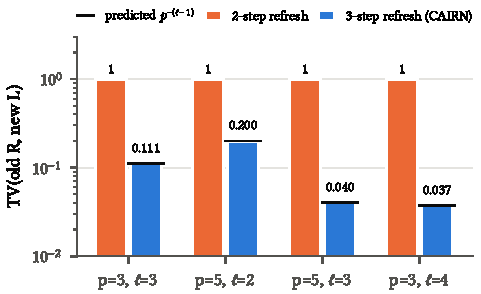
\includegraphics[width=\textwidth]{figures/refresh.pdf}
\caption{Cross-epoch leakage: two-step refresh (orange) leaks the value; \cairn{}'s three-step refresh meets the prediction $p^{-(\ell-1)}$ (black ticks).}\label{fig:refresh}
\end{minipage}\hfill
\begin{minipage}[b]{0.47\textwidth}\centering
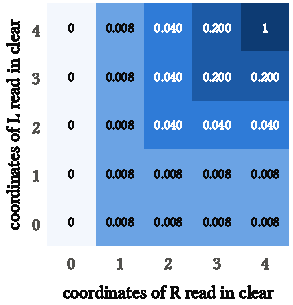
\includegraphics[width=0.66\textwidth]{figures/leakage.pdf}
\caption{Exact advantage over $\F_5$, $\ell=4$, when $a$ coordinates of $L$ and $b$ of $R$ are read in the clear. It is exactly $0$ when $R$ is not read ($b=0$), equals $p^{-(\ell-\max(\min(a,b),1))}$ otherwise, and reaches 1 only when both halves are read in full.}\label{fig:leakage}
\end{minipage}
\end{figure}

\paragraph{Timing.} We follow dudect~\cite{reparaz17}: fixed and random inputs are interleaved in random order, inputs are prepared in advance in one array so both classes execute identical code, and Welch's $t$ is computed on the raw cycle counts and on five percentile crops. On an Intel Core i7-1185G7, \cairn{} shows $\max|t|=\DudectMulCairn$ (multiplication, \SamplesMulCairn{} traces), \DudectInvCairn{} (inversion) and \DudectRecCairn{} (full reconstruction and AMD check), all below the 4.5 threshold, while the textbook baseline (double-and-add multiplication, extended Euclid) shows \DudectMulNaive{}, \DudectInvNaive{} and \DudectRecNaive{} on the same harness (\cref{fig:dudect}). A methodological note: our first harness chose the input with a branch just before the timed region and reported a false positive ($|t|\approx22$) on \cairn{}'s multiplication; moving to dudect's precomputed-input design removed it. We report this because a timing test is only as good as its harness.

\paragraph{ctgrind, assembly and memory safety.} Following Langley~\cite{langley10}, \code{tools/ctgrind.sh} marks share memory as undefined for Valgrind's memcheck, which then reports any branch or address that depends on it; the baseline is the positive control. \code{tools/asm\_audit.sh} disassembles the release binary: multiplication (72 instructions), addition and subtraction (110) and constant-time selection (29) contain no conditional jump and no division; the AMD tag contains exactly two, both on the public limb count. All core unit tests pass under Miri.

\begin{figure}[t]
\centering
\begin{minipage}[b]{0.52\textwidth}\centering
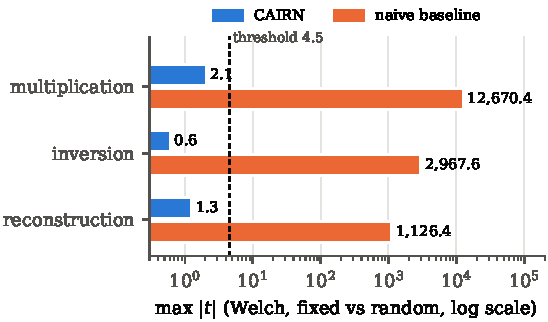
\includegraphics[width=\textwidth]{figures/dudect.pdf}
\caption{Fixed-versus-random Welch test (log scale). Bars below 4.5 show no detectable timing leakage.}\label{fig:dudect}
\end{minipage}\hfill
\begin{minipage}[b]{0.44\textwidth}\centering
\small
\begin{tabular}{@{}lr@{}}
\toprule
operation (32-byte key) & median\\
\midrule
\rows{bench}
\bottomrule
\end{tabular}
\captionof{table}{Performance, one core, i7-1185G7.}\label{tab:bench}
\end{minipage}
\end{figure}

\section{Comparison}\label{sec:comparison}

\Cref{tab:compare} places \cairn{} among classical threshold schemes. Its distinguishing combination is unconditional tamper detection, a leakage model for storage and two levels of refresh, all without a computational assumption and without any pre-existing cipher or hash.

\begin{table}[!htbp]
\centering\small
\begin{tabularx}{\textwidth}{@{}l *{5}{>{\raggedright\arraybackslash}X}@{}}
\toprule
& Shamir~\cite{shamir79} & Feldman VSS~\cite{feldman87} & Pedersen VSS~\cite{pedersen91} & Asmuth-Bloom~\cite{asmuth83} & \cairn{}\\
\midrule
Secrecy & perfect & computational (DL) & perfect & statistical & perfect\\
Tamper detection & none & yes, DL & yes, DL & none & yes, unconditional\\
Leakage model & none & none & none & none & split-state, bounded\\
Refresh & no & extensions & extensions & no & yes, two levels\\
Assumptions & none & discrete log & discrete log & none & none\\
Uses a cipher or hash & no & no & no & no & no\\
\bottomrule
\end{tabularx}
\caption{\cairn{} against classical threshold schemes. VSS schemes additionally let custodians verify their shares against public commitments, which \cairn{} does not provide.}\label{tab:compare}
\end{table}

\section{Limitations}\label{sec:limits}
We state what \cairn{} does \emph{not} do. (1) The dealer and the combiner are trusted while they run; at the moment of use the key exists in the clear in the combiner's memory, in a locked, zeroized buffer, for about \BenchCombine{}. (2) Robustness requires authenticated indices (\cref{prop:keyless}). (3) The leakage theorem bounds leakage from storage; it does not by itself model leakage of the computation that combines both halves, which we address with constant-time code and measurements instead. (4) We did not perform power or electromagnetic measurements on hardware. (5) The multi-epoch cross-refresh analysis beyond one refresh is open (\cref{lem:refresh}). (6) Shares are not publicly verifiable as in VSS. (7) The \code{Copy} field type can leave register or stack copies that zeroization cannot reach; we minimize but cannot exclude them in a high-level language.

\section{Conclusion}
Linear algebra over one Mersenne prime is enough to protect a master key against theft, patience, memory disclosure, timing and lies, with theorems that need no unproven assumption and an implementation whose every claim is reproduced by one command. The most useful finding of our own cryptanalysis is also the simplest: a refresh that looks correct can leak everything across two snapshots, and only an exact analysis, not testing for correctness, reveals it.

\paragraph{Reproducibility.} \code{make verify} runs the lint, unit, property and known-answer tests, the exhaustive lab, the attacks, ctgrind, the assembly audit, regenerates every figure and table in this paper from \code{results/*.json}, and rebuilds this PDF.

\small
\begin{thebibliography}{99}\setlength{\itemsep}{1pt}
\bibitem{asmuth83} C.~Asmuth and J.~Bloom. A modular approach to key safeguarding. \emph{IEEE Trans.\ Inf.\ Theory}, 29(2):208--210, 1983.
\bibitem{blakley79} G.~R.~Blakley. Safeguarding cryptographic keys. In \emph{AFIPS National Computer Conference}, pages 313--317, 1979.
\bibitem{chor88} B.~Chor and O.~Goldreich. Unbiased bits from sources of weak randomness and probabilistic communication complexity. \emph{SIAM J.\ Comput.}, 17(2):230--261, 1988.
\bibitem{cramer08} R.~Cramer, Y.~Dodis, S.~Fehr, C.~Padr\'o and D.~Wichs. Detection of algebraic manipulation with applications to robust secret sharing and fuzzy extractors. In \emph{EUROCRYPT 2008}, LNCS 4965, pages 471--488.
\bibitem{davi10} F.~Dav\`i, S.~Dziembowski and D.~Venturi. Leakage-resilient storage. In \emph{SCN 2010}, LNCS 6280, pages 121--137.
\bibitem{dziembowski11} S.~Dziembowski and S.~Faust. Leakage-resilient cryptography from the inner-product extractor. In \emph{ASIACRYPT 2011}, LNCS 7073, pages 702--721.
\bibitem{feldman87} P.~Feldman. A practical scheme for non-interactive verifiable secret sharing. In \emph{FOCS 1987}, pages 427--437.
\bibitem{halderman08} J.~A.~Halderman et al. Lest we remember: cold boot attacks on encryption keys. In \emph{USENIX Security 2008}.
\bibitem{herzberg95} A.~Herzberg, S.~Jarecki, H.~Krawczyk and M.~Yung. Proactive secret sharing, or: how to cope with perpetual leakage. In \emph{CRYPTO 1995}, LNCS 963, pages 339--352.
\bibitem{kocher96} P.~Kocher. Timing attacks on implementations of Diffie-Hellman, RSA, DSS, and other systems. In \emph{CRYPTO 1996}, LNCS 1109, pages 104--113.
\bibitem{langley10} A.~Langley. ctgrind: checking that functions are constant time with Valgrind. \url{https://github.com/agl/ctgrind}, 2010.
\bibitem{mceliece81} R.~J.~McEliece and D.~V.~Sarwate. On sharing secrets and Reed-Solomon codes. \emph{Commun.\ ACM}, 24(9):583--584, 1981.
\bibitem{ostrovsky91} R.~Ostrovsky and M.~Yung. How to withstand mobile virus attacks. In \emph{PODC 1991}, pages 51--59.
\bibitem{pedersen91} T.~P.~Pedersen. Non-interactive and information-theoretic secure verifiable secret sharing. In \emph{CRYPTO 1991}, LNCS 576, pages 129--140.
\bibitem{reparaz17} O.~Reparaz, J.~Balasch and I.~Verbauwhede. Dude, is my code constant time? In \emph{DATE 2017}, pages 1697--1702.
\bibitem{shamir79} A.~Shamir. How to share a secret. \emph{Commun.\ ACM}, 22(11):612--613, 1979.
\bibitem{tompa88} M.~Tompa and H.~Woll. How to share a secret with cheaters. \emph{J.\ Cryptology}, 1(2):133--138, 1988.
\end{thebibliography}

\end{document}
